\chapter{Expected Sensitivity}
\label{chap:Sensitivity}

Data events in the \acp{SR} of this analysis are still hidden as strategies are still being finalized. Nevertheless, preliminary studies are performed to understand the overall sensitivity, as well as the sensitivity of each event channel. These studies utilize Asimov datasets to reconstruct the likelihood function, which is then used to perform the profile likelihood fit and calculate the upper limits. The Asimov datasets replace data events with background-only template histograms. The one dimensional profile likelihood fit and upper limit is discussed in \autoref{sec:1d}. The two-dimensional likelihood scan is discussed in \autoref{sec:2d}.
%%%%%%%%%%%%%%%%%%%%%%%%%%%%%%%%%%%%%%%%%%%%%%%%%%%%
%%%%%%%%%%%%%%%%%%%%%%%%%%%%%%%%%%%%%%%%%%%%%%%%%%%%

\section{Upper Limits}
\label{sec:1d}

The one-dimensional likelihood function $\mathcal{L}(\mu, \theta)$ is very similar to the one described in \autoref{sec:PLF} with a few notable differences. Firstly, templates are constructed directly from event yields in search bins as \ac{BDT} is not used in this analysis. Secondly, only statistical uncertainties, luminosity uncertainties, and normalization uncertainties of \ac{MC} samples are considered as other systematic uncertainties are still being evaluated. A 20\% normalization uncertainties are assigned to the normalizations of the $\ttbar$ and \ac{DY} backgrounds as they are considered \emph{fake} tau backgrounds with larger uncertainties. A 10\% uncertainty is assigned to the normalizations of signal and other background processes. Lastly, there are three independent signals contained in one sample, and they are used to construct the likelihood functions separately.

The likelihood function is maximized based on the Asimov datasets. Representative impacts of the nuisance parameters on the likelihood fit are shown in Figure~\ref{fig:Impact_2}.

 \begin{figure}[tbh!]
 \begin{center}
 \begin{tabular}{c}
 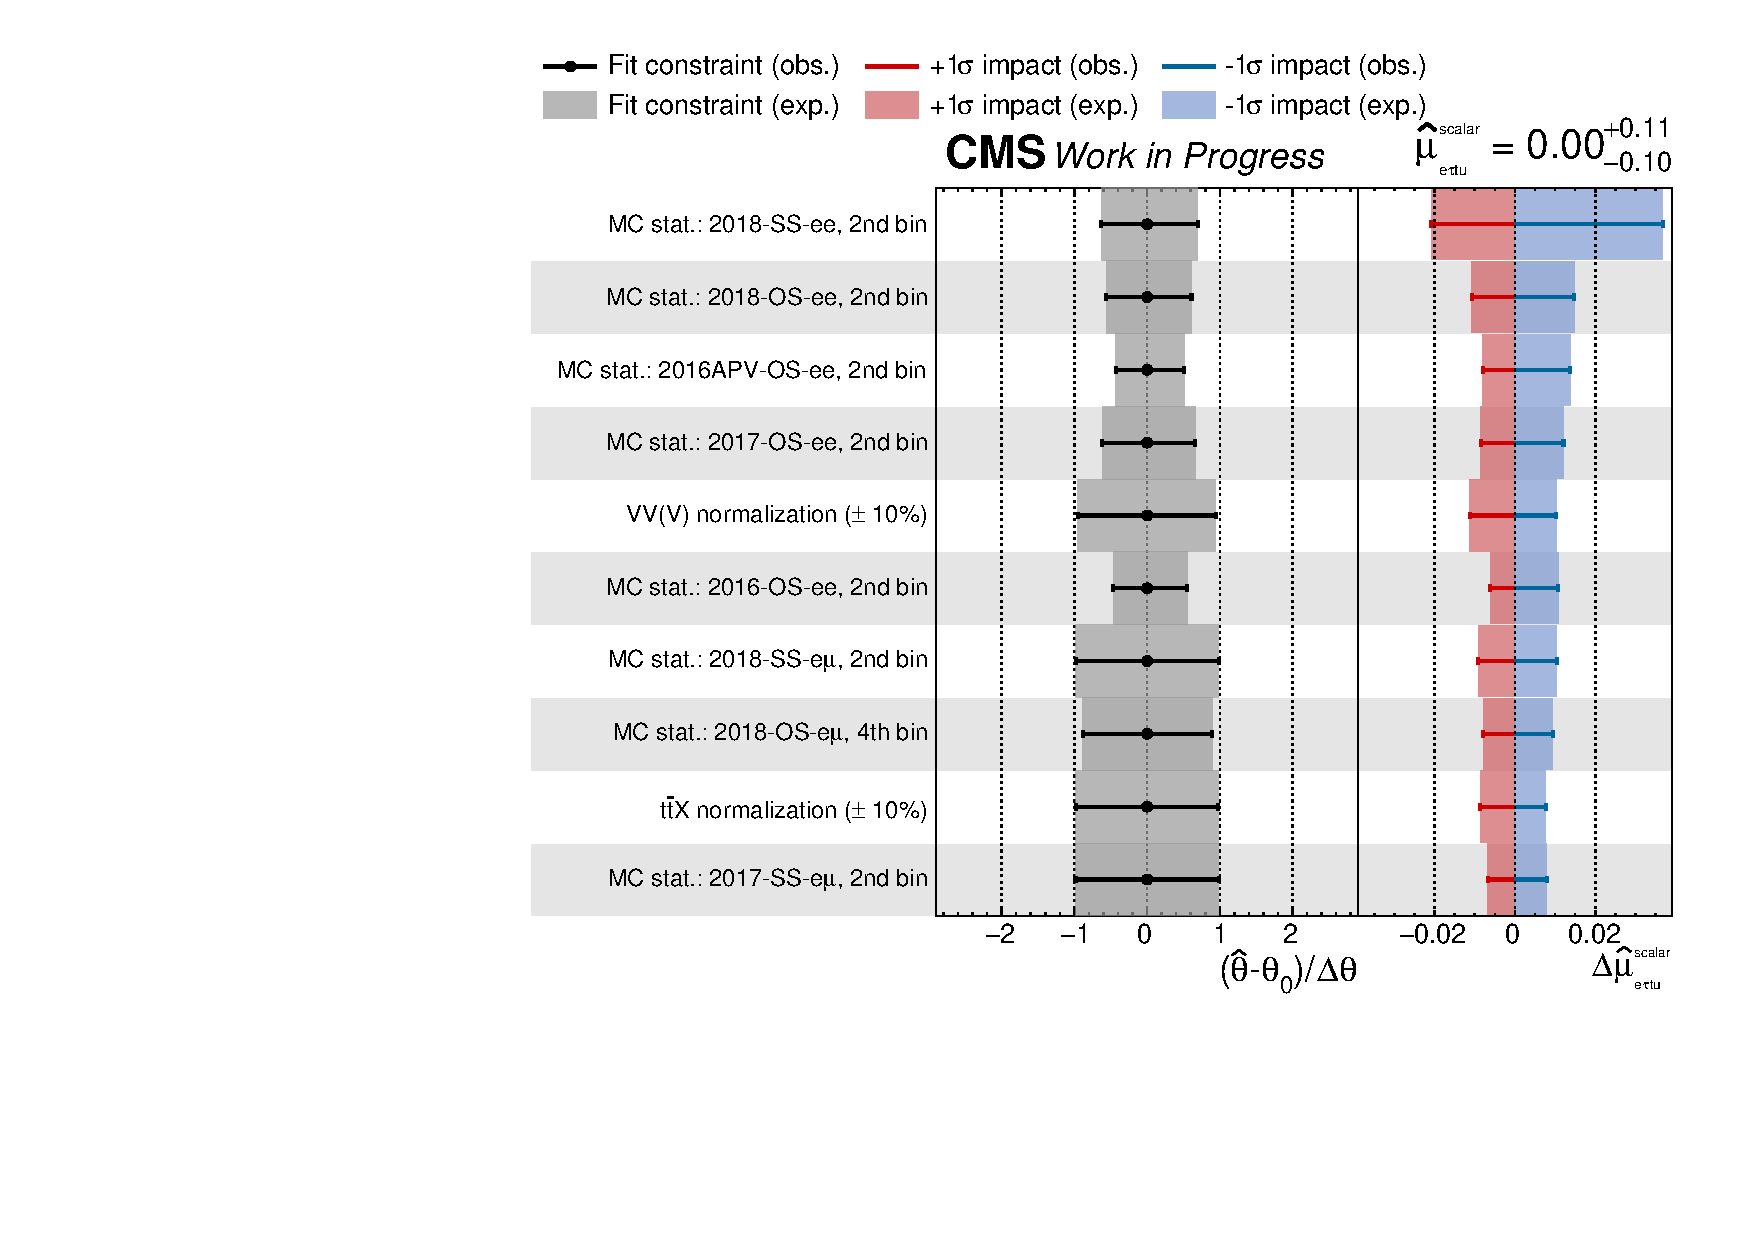
\includegraphics[width=0.9\textwidth]{figures/Part4/Sensitivity/Impact}
 \end{tabular}
 \caption{The nominal value of the expected signal strength $\hat{\mu}$ and its uncertainty is shown in the top right corner. Ranking of the nuisance parameters according to their expected impacts on $\hat{\mu}$ (represented with error bars) is shown in the right panel. Only the 10 nuisance parameters with the largest observed impacts are shown. The impact of each nuisance parameter, $\mathrm{\Delta}\hat{\mu}$, is calculated as the difference between the nominal $\hat{\mu}$ and the value of $\hat{\mu}$ when the corresponding nuisance parameter is fixed to $\hat{\theta}\pm\sigma$, where $\hat{\theta}$ ($\sigma$) is its post-fit value (uncertainty).}
 \label{fig:Impact_2}
 \end{center}
 \end{figure}
 
Using the same limit setting procedure described in \autoref{sec:Limits}, one-dimensional limits at 95\% \ac{CL} can be calculated for each flavor mixing signal. Expected limits on the scalar-like operator involving an up quark are summarized in Table~\ref{tab:limit}.
 
\begin{table}[th]
\sffamily
\centering
\caption{Expected upper limits at 95\% \ac{CL} on \acp{WC} and the branching fractions. The intervals that contain 68\% of the distribution of the expected upper limits are shown in parentheses.}
\resizebox{0.8\linewidth}{!}{%
\begin{tabular}{cccc}
\toprule
CLFV & Event & $\WC{}{\ell\ell^{\prime}\textsf{tu}}/\mathrm{\Lam}^2~(\TeV^{-2})$ & $\mathcal{B} (t \rightarrow \ell\ell^{\prime}\textsf{u}) \times 10^{-6}$ \\
coupling & channel & exp (68\% range) & exp (68\% range) \\
\midrule
\multirow{4}{*}{$\emut{u}$}& SS-e$\upmu$ & 2.23 (2.23--2.23) & 2.23 (2.23--2.23) \\
& SS-$\upmu\upmu$ & 2.02 (2.02--2.02) & 2.02 (2.02--2.02) \\
& OS-e$\upmu$ & 1.09 (1.09--1.09) & 1.09 (1.09--1.09) \\
& Combined & 1.04 (1.04--1.04) & 1.04 (1.04--1.04) \\
\midrule
\multirow{5}{*}{e$\uptau$tu} & OS-es & 1.23 (1.23--1.23) & 1.23 (1.23--1.23) \\
 & OS-e$\upmu$ & 0.93 (0.93--0.93) & 0.93 (0.93--0.93) \\
 & SS-ee & 0.69 (0.69--0.69) & 0.69 (0.69--0.69) \\
 & SS-e$\upmu$ & 0.57 (0.57--0.57) & 0.57 (0.57--0.57) \\
 & Combined & 0.49 (0.49--0.49) & 0.49 (0.49--0.49) \\
 \midrule
\multirow{5}{*}{$\upmu\uptau$tu} & OS-$\upmu\upmu$ & 1.14 (1.14--1.14) & 1.14 (1.14--1.14) \\
 & OS-e$\upmu$ & 0.87 (0.87--0.87) & 0.87 (0.87--0.87) \\
 & SS-e$\upmu$ & 0.54 (0.54--0.54) & 0.54 (0.54--0.54) \\
 & SS-$\upmu\upmu$ & 0.48 (0.48--0.48) & 0.48 (0.48--0.48) \\
 & Combined & 0.41 (0.41--0.41) & 0.41 (0.41--0.41) \\
 \bottomrule
\end{tabular}
}
\label{tab:limit2}
\end{table}

%%%%%%%%%%%%%%%%%%%%%%%%%%%%%%%%%%%%%%%%%%%%%%%%%%%%
%%%%%%%%%%%%%%%%%%%%%%%%%%%%%%%%%%%%%%%%%%%%%%%%%%%%

\section{Two Dimensional Likelihood Scan}
\label{sec:2d}

The two-dimensional likelihood function $\mathcal{L}(\mu_1, \mu_2, \theta)$ is constructed by injecting two signals simultaneously. The $\mu_1$ and $\mu_2$ correspond to signal strengths of signals generated in different flavor mixing modes. For a given pair of signal strengths ($\mu_1$, $\mu_1$), nuisance parameters $\theta$ are profile to achieve the maximum likelihood, denoted by $\mathcal{L}(\mu_1, \mu_2, \hat{\theta}_{\mu_1,\mu_2})$. This process is repeated to scan through the $\mu_1$-$\mu_1$ space. The results of the profiled likelihood at each point in $\mu_1$-$\mu_1$ space are then compared with the expected likelihood distribution to locate the boundaries of the 68\% and 90\% ranges, which are shown in Figure~\ref{fig:2DScan}.

 \begin{figure}[tbh!]
 \begin{center}
 \begin{tabular}{ccc}
 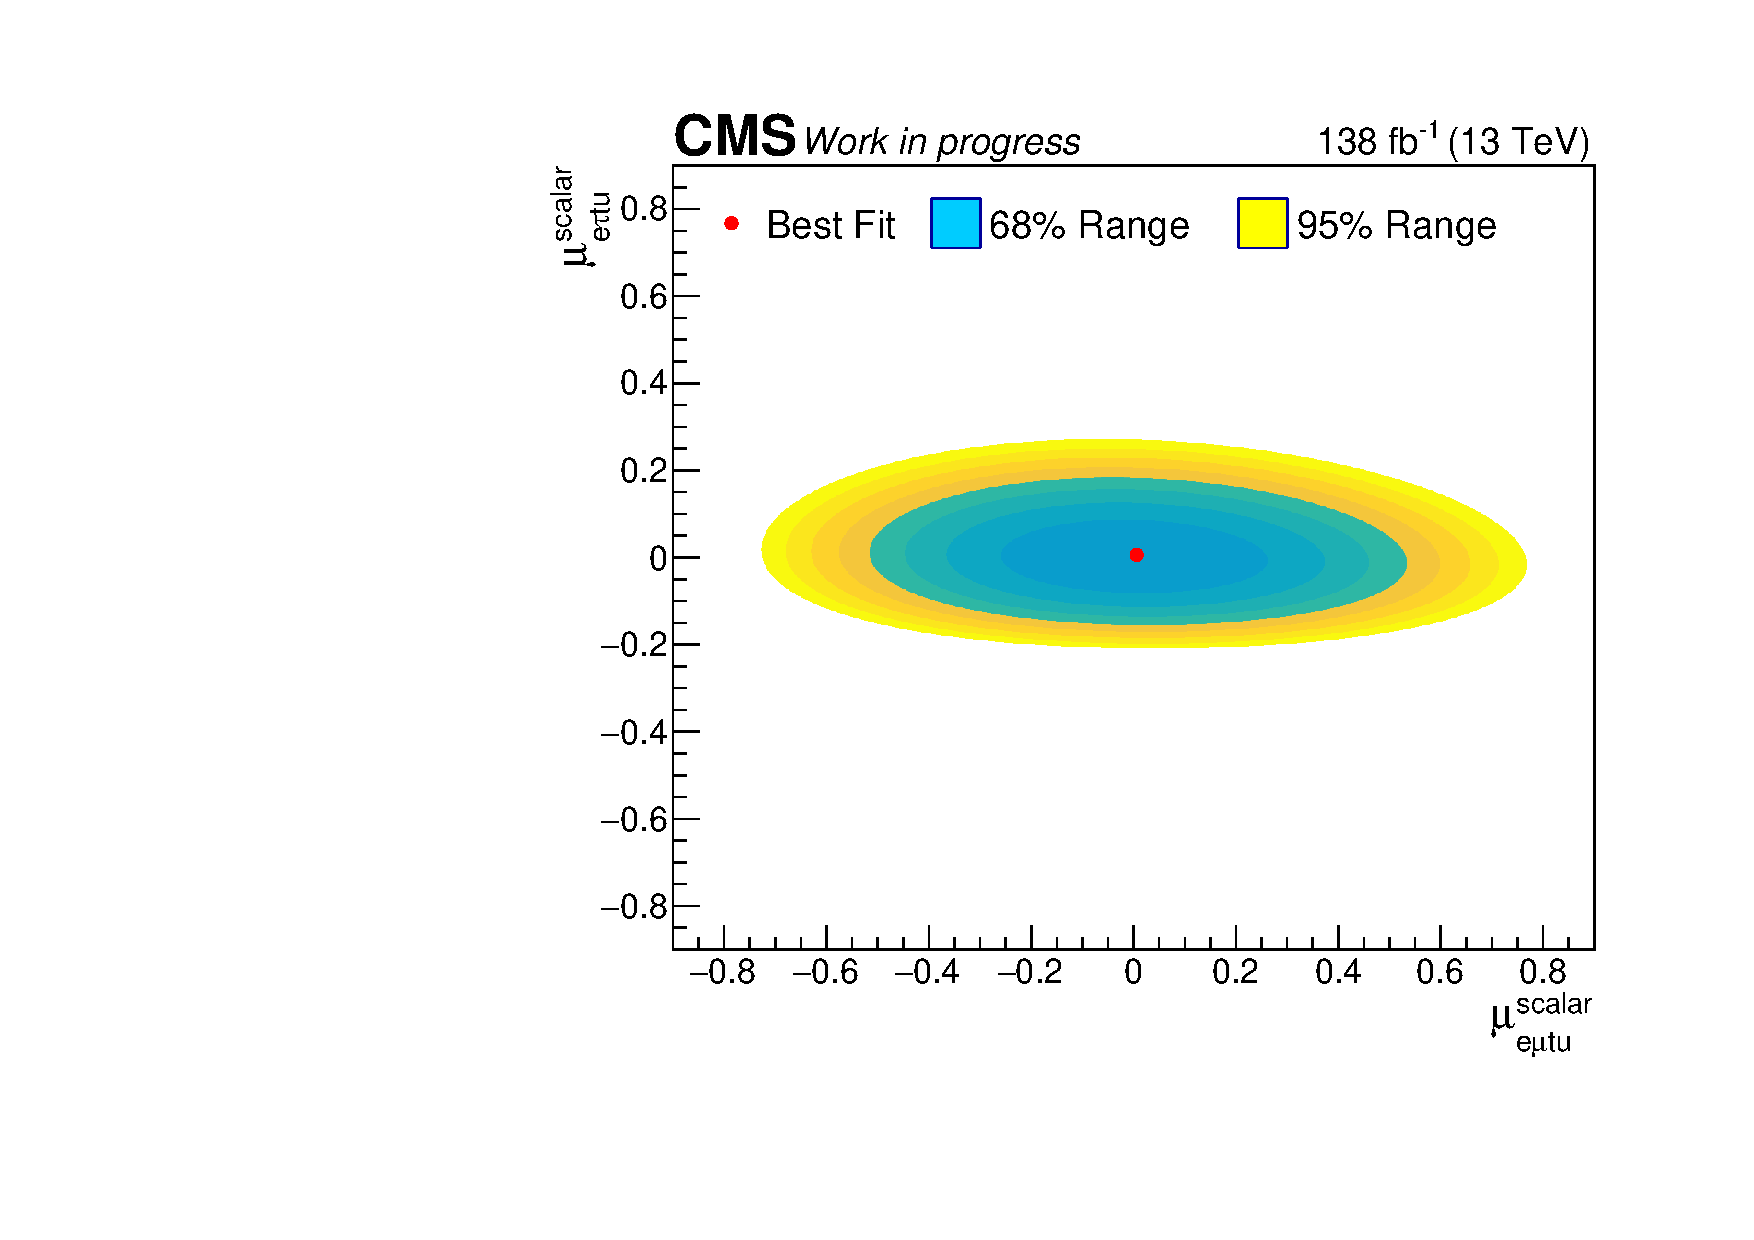
\includegraphics[width=0.33\textwidth]{figures/Part4/Sensitivity/2dScan_emuetau}&
 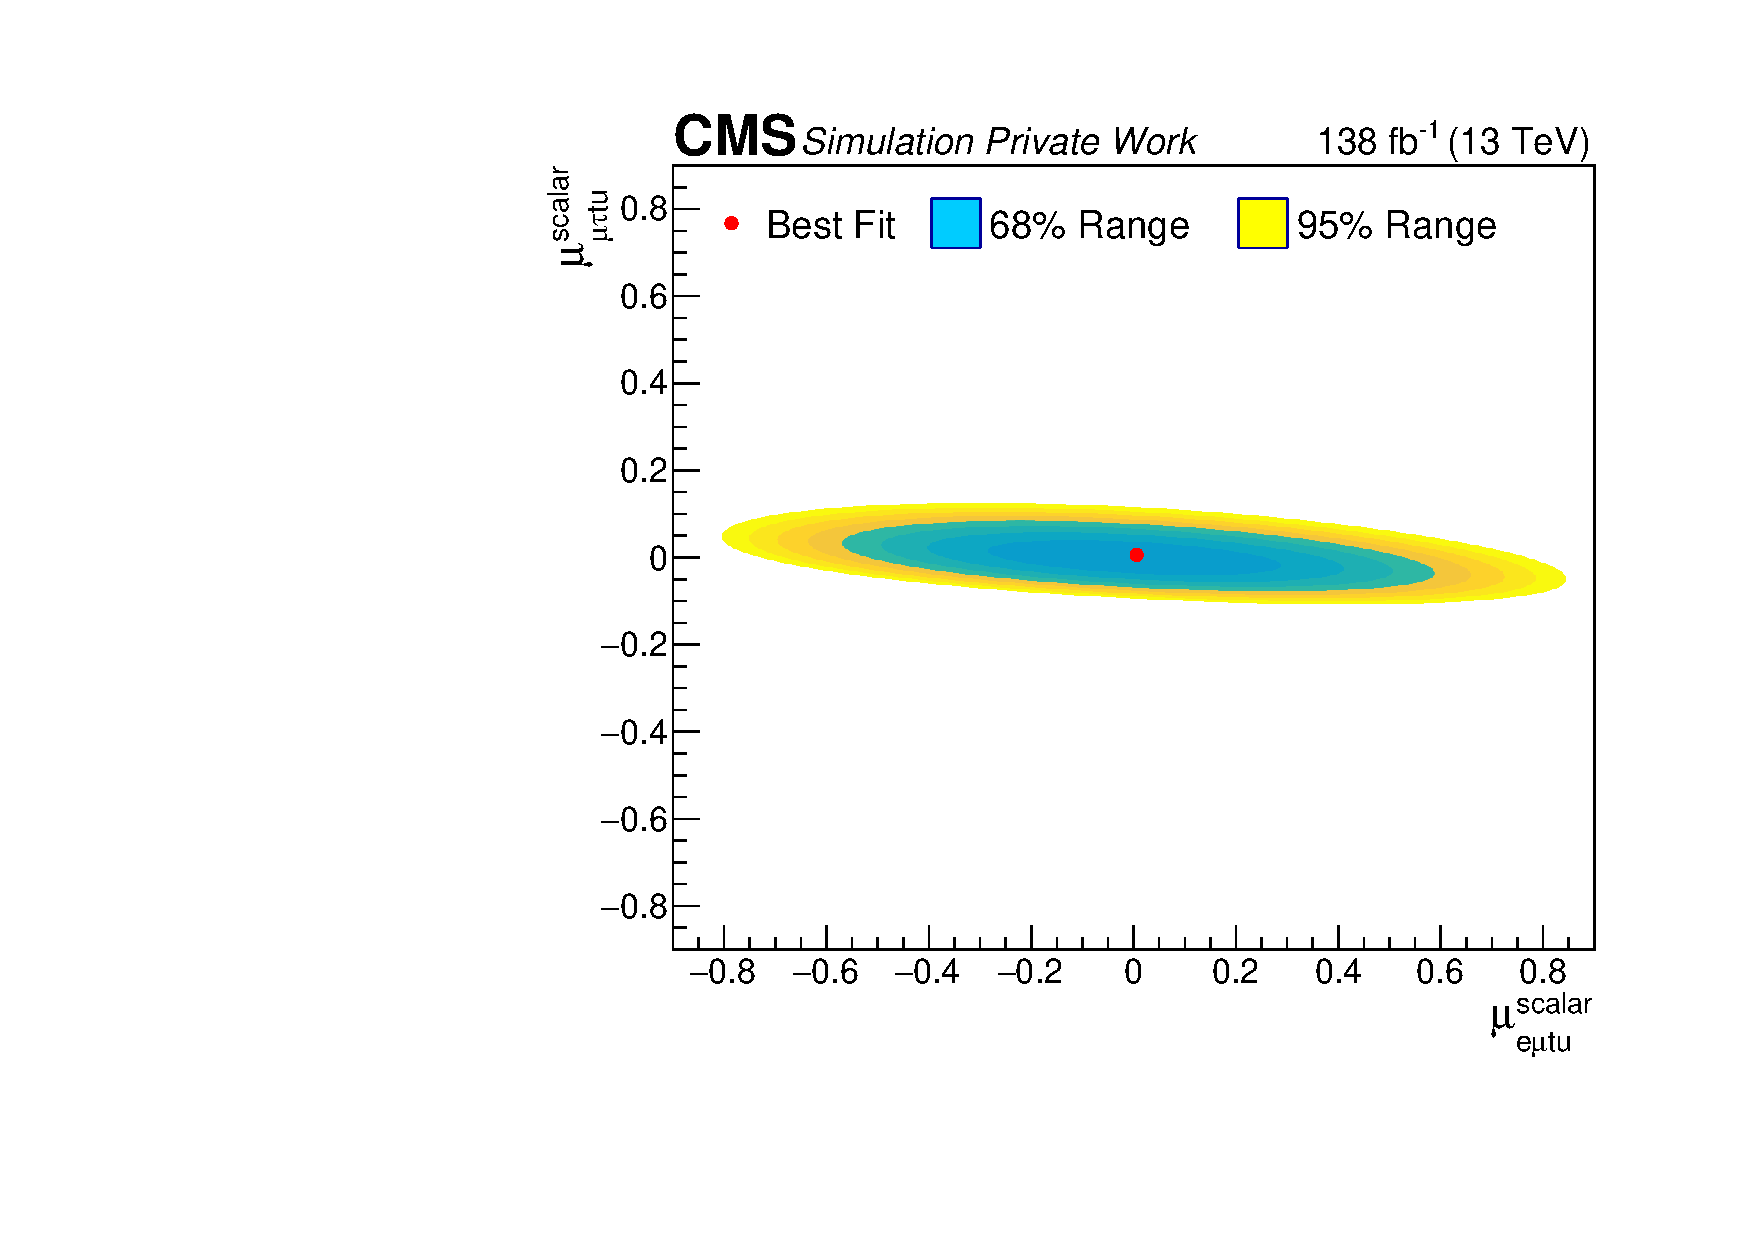
\includegraphics[width=0.33\textwidth]{figures/Part4/Sensitivity/2dScan_emumutau}&
 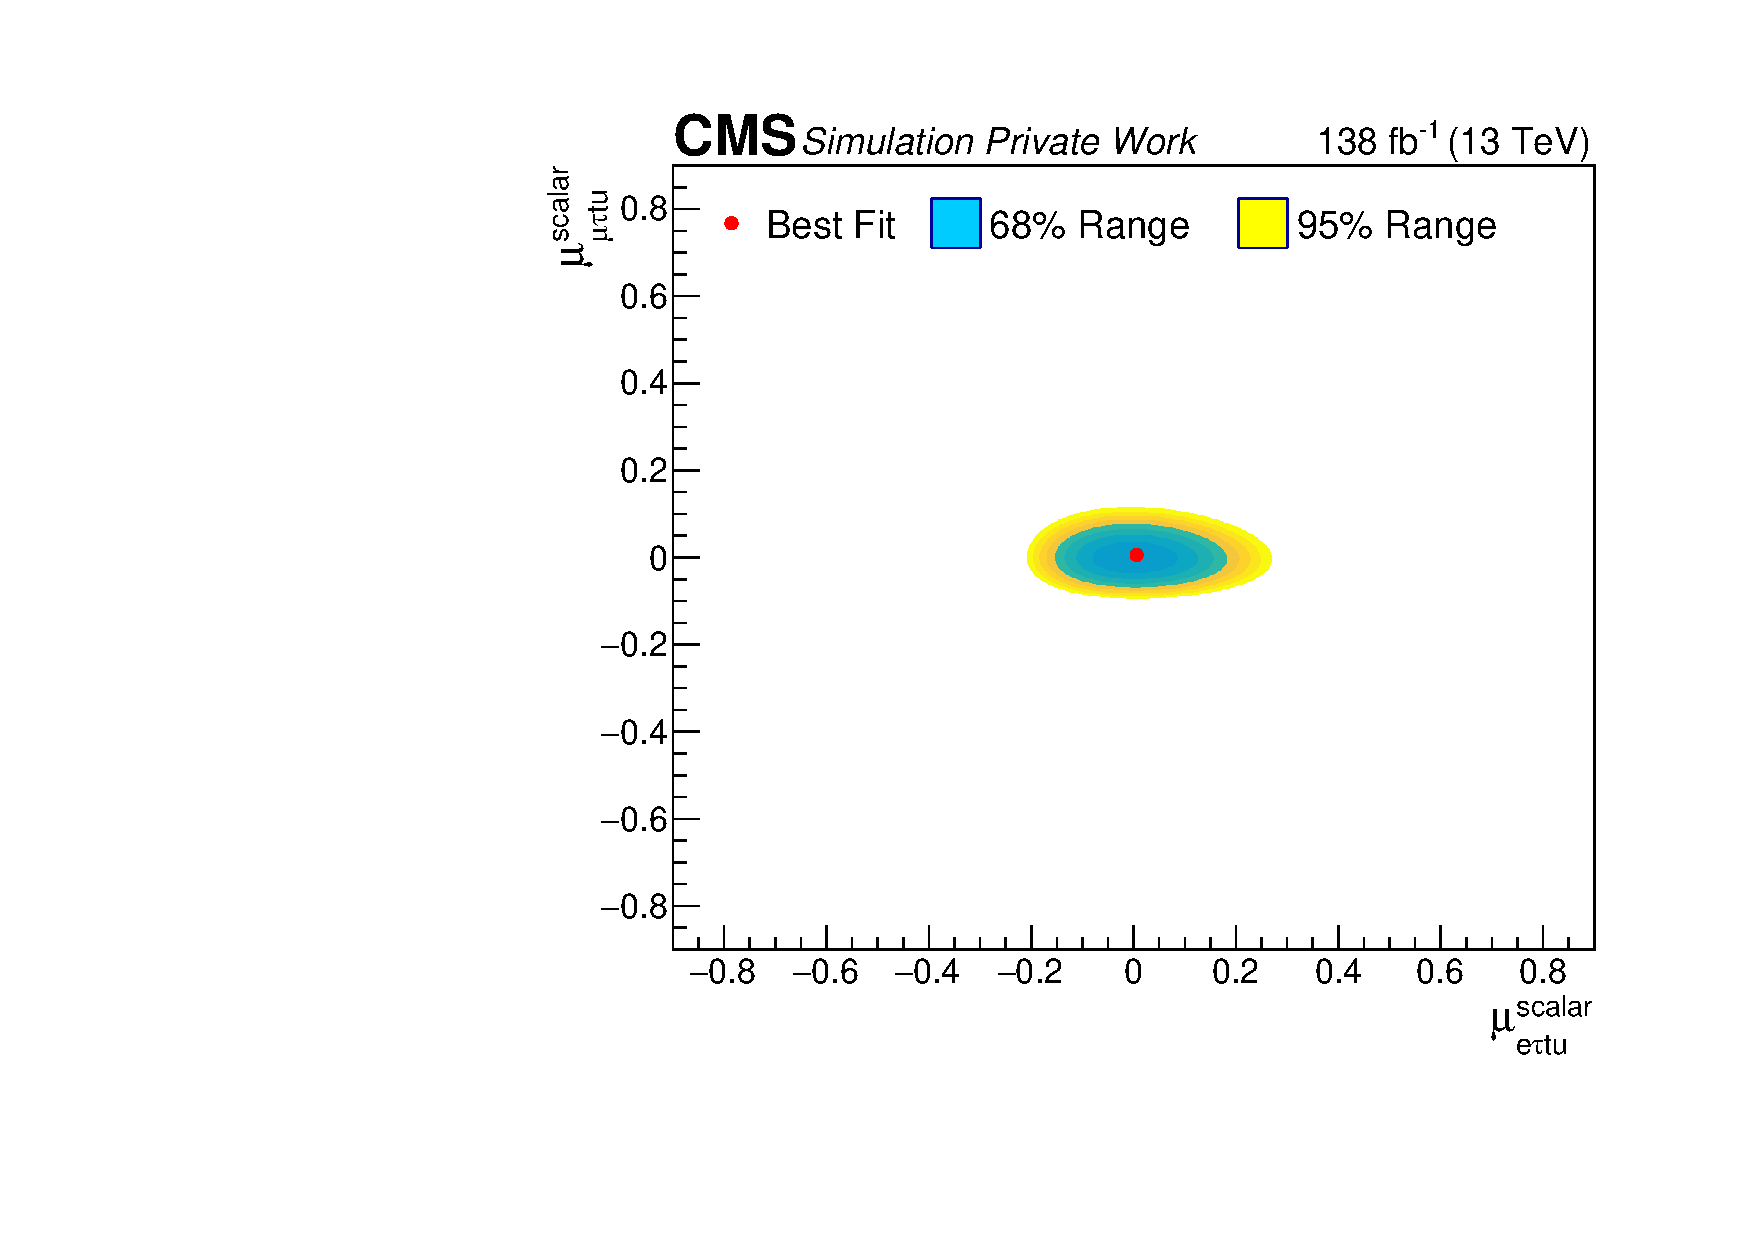
\includegraphics[width=0.33\textwidth]{figures/Part4/Sensitivity/2dScan_etaumutau}\\
 \end{tabular}
 \caption{Two dimensional likelihood scans performed in the e$\upmu$-e$\uptau$ (left), e$\upmu$-$\upmu\uptau$ (middle), and e$\uptau$-$\upmu\uptau$ (right) spaces.}
 \label{fig:2DScan}
 \end{center}
 \end{figure}